\documentclass[border=3mm,tikz,preview]{standalone}
\usepackage[utf8]{inputenc}
\usepackage{amsmath,amssymb,amsfonts}
\usepackage{graphicx}
\usepackage{tikz}
\usetikzlibrary{shapes.geometric, arrows.meta, positioning, shadows, calc, fit, backgrounds}
\usepackage{xcolor}
\begin{document}

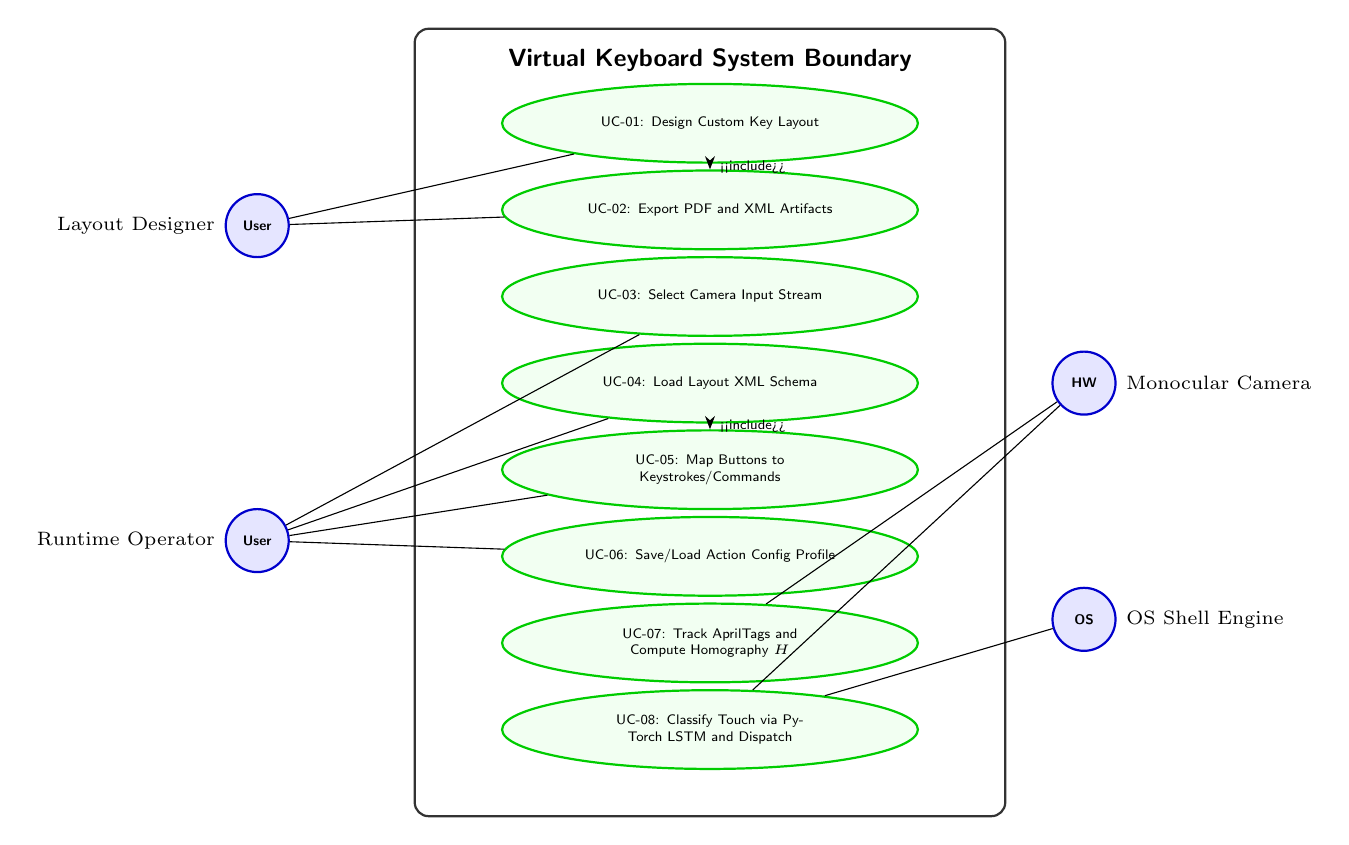
\begin{tikzpicture}[
    actor/.style = {circle, draw=blue!80!black, fill=blue!10!white, thick, minimum size=0.8cm, font=\sffamily\bfseries\tiny},
    usecase/.style = {ellipse, draw=green!80!black, fill=green!5!white, thick, align=center, font=\sffamily\tiny, minimum width=3.8cm, minimum height=1.0cm, text width=3.5cm}
]

% System Boundary
\draw [black!80, thick, rounded corners=5pt] (-1.5,-5.5) rectangle (6,4.5);
\node at (2.25, 4.1) [font=\sffamily\bfseries\small] {Virtual Keyboard System Boundary};

% Actors
\node (designer_actor) [actor, label=left:{\scriptsize Layout Designer}] at (-3.5, 2) {User};
\node (operator_actor) [actor, label=left:{\scriptsize Runtime Operator}] at (-3.5, -2) {User};
\node (camera_actor) [actor, label=right:{\scriptsize Monocular Camera}] at (7, 0) {HW};
\node (os_actor) [actor, label=right:{\scriptsize OS Shell Engine}] at (7, -3) {OS};

% Use Cases App 1
\node (uc1) [usecase] at (2.25, 3.3) {UC-01: Design Custom Key Layout};
\node (uc2) [usecase] at (2.25, 2.2) {UC-02: Export PDF and XML Artifacts};

% Use Cases App 2 Setup
\node (uc3) [usecase] at (2.25, 1.1) {UC-03: Select Camera Input Stream};
\node (uc4) [usecase] at (2.25, 0) {UC-04: Load Layout XML Schema};
\node (uc5) [usecase] at (2.25, -1.1) {UC-05: Map Buttons to Keystrokes/Commands};
\node (uc6) [usecase] at (2.25, -2.2) {UC-06: Save/Load Action Config Profile};

% Use Cases App 2 Runtime
\node (uc7) [usecase] at (2.25, -3.3) {UC-07: Track AprilTags and Compute Homography $H$};
\node (uc8) [usecase] at (2.25, -4.4) {UC-08: Classify Touch via PyTorch LSTM and Dispatch};

% Connections
\draw (designer_actor) -- (uc1);
\draw (designer_actor) -- (uc2);

\draw (operator_actor) -- (uc3);
\draw (operator_actor) -- (uc4);
\draw (operator_actor) -- (uc5);
\draw (operator_actor) -- (uc6);

\draw (camera_actor) -- (uc7);
\draw (camera_actor) -- (uc8);
\draw (os_actor) -- (uc8);

\draw [dashed, ->, >=Stealth] (uc1) -- node[right, font=\sffamily\tiny]{<<include>>} (uc2);
\draw [dashed, ->, >=Stealth] (uc4) -- node[right, font=\sffamily\tiny]{<<include>>} (uc5);

\end{tikzpicture}

\end{document}
